\chapter{activeobjects}
\label{sec:activeobjects}
\lstset{style=68KStyle}
\lhead[tempest 2000]{}

\icode{activeobjects} is a master list of every in-game object on the screen at a given time, with the
exception of the player's claw. It makes sense to keep everything in a list like this and have each
entry tell us what the game should do with the object, where it should draw it, what type of object
it is, and so on. The best way of understanding the use of the \icode{activobjects} list is to see it
in action. To do that, we're going to take a look at a snapshot from a game and examine its full 
\icode{activeobjects} list.

Before we do that, let's take a quick look at what a typical entry in the \icode{activeobjects} list 
looks like. Each entry in the \icode{activeobjects} list is 64 bytes long. Depending on how many bytes we
want to use for each property in an object we could define anything from 16
to 64 properties. In practice, Tempest 2000 has a total of 21 properties, some are 4 bytes (a \icode{long}),
others are 2 bytes (a \icode{word}).

Below we show a typical entry for a player's bullet. 
\begin{figure}[H]
  {
    \setlength{\tabcolsep}{3.0pt}
    \setlength\cmidrulewidth{\heavyrulewidth} % Make cmidrule = 
    \begin{adjustbox}{center}
      \begin{tabular}[t]{ll}
        \toprule
        Bullet & Object Data \\
        \midrule
        \makecell[l]{
            
\includegraphics[width=2.2cm]{activeobjects/bullet.png} \\
        }
        &
        \makecell[l]{
          \begingroup
          \renewcommand{\arraystretch}{.8} % Default value: 1
          \begin{tabular}[t]{ll}
            \tcode{Draw Routine: draw\_pixex}   &    \tcode{YX in Sprite Sheet: 00b6000a}  \\
            \tcode{X: -22}   &    \tcode{Colour: 0078}  \\
            \tcode{Y: -12}   &    \tcode{Scale factor: 0001}  \\
            \tcode{Z: 47}   &    \tcode{0 = climb rail, 1 = cross rail, 2 = blowaway: 0000}  \\
            \tcode{Web Lane: 2}   &    \tcode{Width/Height in Sprite Sheet: 00070007}  \\
            \tcode{Velocity: 1}   &    \tcode{Marked for deletion: 0000}  \\
            \tcode{Acceleration: 0000ca7e}   &    \tcode{Enemy or Not: not an enemy}  \\
            \tcode{Roll: 40}   &    \tcode{run\_vex routine: player\_shot}  \\
            \tcode{Pitch: 0}   &    \tcode{Address of Previous Object: ffffffff}  \\
            \tcode{Yaw: 0}   &    \tcode{Address of Next Object: 0000cc38}  \\
            \tcode{draw\_vex routine: draw\_pixex}   &    \tcode{Current Address: 0xcc78}  \\
          \end{tabular}
          \endgroup
        }
        \\
        \bottomrule
      \end{tabular}
    \end{adjustbox}
  }
\end{figure}

As you can imagine there are usually a few of these. If you take a look at the components included
in the 64 bytes of data representing the object you will see there are a few things whose utility
is obvious: we give the \icode{X}, \icode{Y}, and \icode{Z} co-ordinates of the object; which lane
it is on, its velocity, and its colour. Some others might seem a bit more recherche: roll, pitch,
and yaw, for example, define the angle and shear we apply to the object when drawing it in 3D space. Another
way of describing this is the degree of tilt we apply in the X,Y, and Z directions when drawing the object.
The most obscure-looking of all are the various 'routines' associated with the object. In the example given
above we can see that the routines \icode{draw\_pixex} and \icode{player\_shot} are defined as properties. These
are routines that the game will run when either drawing or updating the state of the object. Lastly we can see
that the object contains addresses for the next and previou objects in the list. This is a useful feature
when reading the \icode{activeobjects} list - they tell us that when we're finishing processing this particular
\icode{activeobject}, which object we should jump to next.

So let's take a look at a random game screen and enumerate the \icode{activeobject} list associated with it.
We've chosen a rather busy screen:
\begin{figure}[H]
    \centering
    \frame{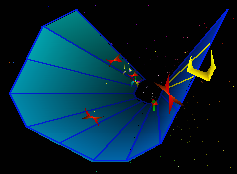
\includegraphics[width=11cm]{src/activeobjects/data_1_raw.png}}%
  \caption{Our random screen.}
\end{figure}

Let's enumerate the entire \icode{activeobjects} list for this screen to give us an idea of how much is being managed 
at once. We give the objects in the order in which they appear in the list.

\begin{figure}[H]
  {
    \setlength{\tabcolsep}{3.0pt}
    \setlength\cmidrulewidth{\heavyrulewidth} % Make cmidrule = 
    \begin{adjustbox}{center}
      \begin{tabular}[t]{ll}
  \toprule
        Enemy Bullet & Object Data \\
        \midrule
        \makecell[l]{
            
\includegraphics[width=2.2cm]{activeobjects/chevron.png} \\
        }
        &
        \makecell[l]{
          \begingroup
          \renewcommand{\arraystretch}{.8} % Default value: 1
          \begin{tabular}[t]{ll}
\tcode{Draw Routine: s\_shot}   &    \tcode{Y/X in Sprite Sheet: 00b6000a}  \\
\tcode{X: -12}   &    \tcode{Colour: 0018}  \\
\tcode{Y: -26}   &    \tcode{Scale factor: 0000}  \\
\tcode{Z: 100}   &    \tcode{0 = climb rail, 1 = cross rail, 2 = blowaway: 0000}  \\
\tcode{Web Lane: 0}   &    \tcode{Width/Height in Sprite Sheet: 00070007}  \\
\tcode{Velocity: 0}   &    \tcode{Marked for deletion: 0000}  \\
\tcode{Acceleration: 0000ca82}   &    \tcode{Enemy or Not: enemy}  \\
\tcode{Roll: 124}   &    \tcode{run\_vex routine: run\_ashot}  \\
\tcode{Pitch: 0}   &    \tcode{Address of Previous Object: ffffffff}  \\
\tcode{Yaw: 0}   &    \tcode{Address of Next Object: 0000d038}  \\
\tcode{draw\_vex routine: draw}   &    \tcode{Current Address: 0xcbf8}  \\
          \end{tabular}
          \endgroup
        }
        \\
        \toprule
        Player Bullet & Object Data \\
        \midrule
        \makecell[l]{
            
\includegraphics[width=2.2cm]{activeobjects/bullet.png} \\
        }
        &
        \makecell[l]{
          \begingroup
          \renewcommand{\arraystretch}{.8} % Default value: 1
          \begin{tabular}[t]{ll}
\tcode{Draw Routine: draw\_pixex}   &    \tcode{Y/X in Sprite Sheet: 00b6000a}  \\
\tcode{X: 22}   &    \tcode{Colour: 0058}  \\
\tcode{Y: -16}   &    \tcode{Scale factor: 0001}  \\
\tcode{Z: 194}   &    \tcode{0 = climb rail, 1 = cross rail, 2 = blowaway: 0000}  \\
\tcode{Web Lane: 10}   &    \tcode{Width/Height in Sprite Sheet: 00070007}  \\
\tcode{Velocity: 1}   &    \tcode{Marked for deletion: ffff}  \\
\tcode{Acceleration: 0000ca6e}   &    \tcode{Enemy or Not: not an enemy}  \\
\tcode{Roll: 376}   &    \tcode{run\_vex routine: player\_shot}  \\
\tcode{Pitch: 0}   &    \tcode{Address of Previous Object: 0000cdf8}  \\
\tcode{Yaw: 0}   &    \tcode{Address of Next Object: 0000cd38}  \\
\tcode{draw\_vex routine: draw\_pixex}   &    \tcode{Current Address: 0xcc38}  \\
          \end{tabular}
          \endgroup
        }
        \\
        \toprule
        Player Bullet & Object Data \\
        \midrule
        \makecell[l]{
            
\includegraphics[width=2.2cm]{activeobjects/bullet.png} \\
        }
        &
        \makecell[l]{
          \begingroup
          \renewcommand{\arraystretch}{.8} % Default value: 1
          \begin{tabular}[t]{ll}
\tcode{Draw Routine: draw\_pixex}   &    \tcode{Y/X in Sprite Sheet: 00b6000a}  \\
\tcode{X: 26}   &    \tcode{Colour: 0028}  \\
\tcode{Y: -24}   &    \tcode{Scale factor: 0001}  \\
\tcode{Z: 191}   &    \tcode{0 = climb rail, 1 = cross rail, 2 = blowaway: 0000}  \\
\tcode{Web Lane: 11}   &    \tcode{Width/Height in Sprite Sheet: 00070007}  \\
\tcode{Velocity: 1}   &    \tcode{Marked for deletion: ffff}  \\
\tcode{Acceleration: 0000ca72}   &    \tcode{Enemy or Not: not an enemy}  \\
\tcode{Roll: 368}   &    \tcode{run\_vex routine: player\_shot}  \\
\tcode{Pitch: 0}   &    \tcode{Address of Previous Object: 0000ccf8}  \\
\tcode{Yaw: 0}   &    \tcode{Address of Next Object: 0000d0b8}  \\
\tcode{draw\_vex routine: draw\_pixex}   &    \tcode{Current Address: 0xcc78}  \\
          \end{tabular}
          \endgroup
        }
        \\
        \bottomrule
      \end{tabular}
    \end{adjustbox}
  }
\end{figure}

\begin{figure}[H]
  {
    \setlength{\tabcolsep}{3.0pt}
    \setlength\cmidrulewidth{\heavyrulewidth} % Make cmidrule = 
    \begin{adjustbox}{center}
      \begin{tabular}[t]{ll}
        \toprule
        Player Bullet & Object Data \\
        \midrule
        \makecell[l]{
            
\includegraphics[width=2.2cm]{activeobjects/bullet.png} \\
        }
        &
        \makecell[l]{
          \begingroup
          \renewcommand{\arraystretch}{.8} % Default value: 1
          \begin{tabular}[t]{ll}
\tcode{Draw Routine: draw\_pixex}   &    \tcode{Y/X in Sprite Sheet: 00b6000a}  \\
\tcode{X: 26}   &    \tcode{Colour: 0028}  \\
\tcode{Y: -24}   &    \tcode{Scale factor: 0001}  \\
\tcode{Z: 191}   &    \tcode{0 = climb rail, 1 = cross rail, 2 = blowaway: 0000}  \\
\tcode{Web Lane: 11}   &    \tcode{Width/Height in Sprite Sheet: 00070007}  \\
\tcode{Velocity: 1}   &    \tcode{Marked for deletion: ffff}  \\
\tcode{Acceleration: 0000ca76}   &    \tcode{Enemy or Not: not an enemy}  \\
\tcode{Roll: 368}   &    \tcode{run\_vex routine: player\_shot}  \\
\tcode{Pitch: 0}   &    \tcode{Address of Previous Object: 0000d078}  \\
\tcode{Yaw: 0}   &    \tcode{Address of Next Object: 0000ccf8}  \\
\tcode{draw\_vex routine: draw\_pixex}   &    \tcode{Current Address: 0xccb8}  \\
          \end{tabular}
          \endgroup
        }
        \\
        \toprule
        Player Bullet & Object Data \\
        \midrule
        \makecell[l]{
            
\includegraphics[width=2.2cm]{activeobjects/bullet.png} \\
        }
        &
        \makecell[l]{
          \begingroup
          \renewcommand{\arraystretch}{.8} % Default value: 1
          \begin{tabular}[t]{ll}
\tcode{Draw Routine: draw\_pixex}   &    \tcode{Y/X in Sprite Sheet: 00b6000a}  \\
\tcode{X: 26}   &    \tcode{Colour: 0028}  \\
\tcode{Y: -24}   &    \tcode{Scale factor: 0001}  \\
\tcode{Z: 191}   &    \tcode{0 = climb rail, 1 = cross rail, 2 = blowaway: 0000}  \\
\tcode{Web Lane: 11}   &    \tcode{Width/Height in Sprite Sheet: 00070007}  \\
\tcode{Velocity: 1}   &    \tcode{Marked for deletion: ffff}  \\
\tcode{Acceleration: 0000ca7a}   &    \tcode{Enemy or Not: not an enemy}  \\
\tcode{Roll: 368}   &    \tcode{run\_vex routine: player\_shot}  \\
\tcode{Pitch: 0}   &    \tcode{Address of Previous Object: 0000ccb8}  \\
\tcode{Yaw: 0}   &    \tcode{Address of Next Object: 0000cc78}  \\
\tcode{draw\_vex routine: draw\_pixex}   &    \tcode{Current Address: 0xccf8}  \\
          \end{tabular}
          \endgroup
        }
        \\
        \toprule
        Player Bullet & Object Data \\
        \midrule
        \makecell[l]{
            
\includegraphics[width=2.2cm]{activeobjects/bullet.png} \\
        }
        &
        \makecell[l]{
          \begingroup
          \renewcommand{\arraystretch}{.8} % Default value: 1
          \begin{tabular}[t]{ll}
\tcode{Draw Routine: draw\_pixex}   &    \tcode{Y/X in Sprite Sheet: 00b6000a}  \\
\tcode{X: 22}   &    \tcode{Colour: 0058}  \\
\tcode{Y: -16}   &    \tcode{Scale factor: 0001}  \\
\tcode{Z: 194}   &    \tcode{0 = climb rail, 1 = cross rail, 2 = blowaway: 0000}  \\
\tcode{Web Lane: 10}   &    \tcode{Width/Height in Sprite Sheet: 00070007}  \\
\tcode{Velocity: 1}   &    \tcode{Marked for deletion: ffff}  \\
\tcode{Acceleration: 0000ca7e}   &    \tcode{Enemy or Not: not an enemy}  \\
\tcode{Roll: 376}   &    \tcode{run\_vex routine: player\_shot}  \\
\tcode{Pitch: 0}   &    \tcode{Address of Previous Object: 0000cc38}  \\
\tcode{Yaw: 0}   &    \tcode{Address of Next Object: 0000cb78}  \\
\tcode{draw\_vex routine: draw\_pixex}   &    \tcode{Current Address: 0xcd38}  \\
          \end{tabular}
          \endgroup
        }
        \\
        \toprule
        Flipper & Object Data \\
        \midrule
        \makecell[l]{
            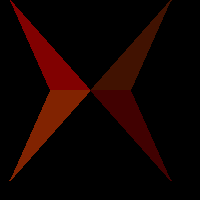
\includegraphics[width=2.2cm]{activeobjects/flipper.png} \\
        }
        &
        \makecell[l]{
          \begingroup
          \renewcommand{\arraystretch}{.8} % Default value: 1
          \begin{tabular}[t]{ll}
\tcode{Draw Routine: cdraw\_sflipper}   &    \tcode{Start address of pixel data.: fff70006}  \\
\tcode{X: 4}   &    \tcode{Colour: 00f0}  \\
\tcode{Y: 8}   &    \tcode{Scale factor: 0001}  \\
\tcode{Z: 30}   &    \tcode{0 = climb rail, 1 = cross rail, 2 = blowaway: 0000}  \\
\tcode{Position/lane on web.: 7}   &    \tcode{Size of Pixel Data: c9ce0007}  \\
\tcode{Velocity: 4}   &    \tcode{Marked for deletion: 0000}  \\
\tcode{Acceleration/Flipper Mode: 00010808}   &    \tcode{Enemy or Not: enemy}  \\
\tcode{XZ Orientation  (Roll): 96}   &    \tcode{run\_vex routine: run\_flipper}  \\
\tcode{Y Rotation  (Pitch): 0}   &    \tcode{Address of Previous Object: 0000cdb8}  \\
\tcode{Z Rotation  (Yaw): 0}   &    \tcode{Address of Next Object: 0000cb38}  \\
\tcode{draw\_vex routine: draw\_vxc}   &    \tcode{Current Address: 0xcd78}  \\
          \end{tabular}
          \endgroup
        }
        \\
        \bottomrule
      \end{tabular}
    \end{adjustbox}
  }
\end{figure}

\begin{figure}[H]
  {
    \setlength{\tabcolsep}{3.0pt}
    \setlength\cmidrulewidth{\heavyrulewidth} % Make cmidrule = 
    \begin{adjustbox}{center}
      \begin{tabular}[t]{ll}
        \toprule
        Flipper & Object Data \\
        \midrule
        \makecell[l]{
            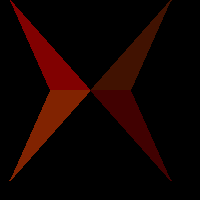
\includegraphics[width=2.2cm]{activeobjects/flipper.png} \\
        }
        &
        \makecell[l]{
          \begingroup
          \renewcommand{\arraystretch}{.8} % Default value: 1
          \begin{tabular}[t]{ll}
\tcode{Draw Routine: cdraw\_sflipper}   &    \tcode{Start address of pixel data.: fff70008}  \\
\tcode{X: 16}   &    \tcode{Colour: 00f0}  \\
\tcode{Y: -4}   &    \tcode{Scale factor: 0001}  \\
\tcode{Z: 30}   &    \tcode{0 = climb rail, 1 = cross rail, 2 = blowaway: 0000}  \\
\tcode{Position/lane on web.: 9}   &    \tcode{Size of Pixel Data: c9ca0101}  \\
\tcode{Velocity: 4}   &    \tcode{Marked for deletion: 0000}  \\
\tcode{Acceleration/Flipper Mode: 00010808}   &    \tcode{Enemy or Not: enemy}  \\
\tcode{XZ Orientation  (Roll): 36}   &    \tcode{run\_vex routine: run\_flipper}  \\
\tcode{Y Rotation  (Pitch): 0}   &    \tcode{Address of Previous Object: 0000ce38}  \\
\tcode{Z Rotation  (Yaw): 0}   &    \tcode{Address of Next Object: 0000cd78}  \\
\tcode{draw\_vex routine: draw\_vxc}   &    \tcode{Current Address: 0xcdb8}  \\
          \end{tabular}
          \endgroup
        }
        \\
        \toprule
        Enemy Bullet & Object Data \\
        \midrule
        \makecell[l]{
            
\includegraphics[width=2.2cm]{activeobjects/chevron.png} \\
        }
        &
        \makecell[l]{
          \begingroup
          \renewcommand{\arraystretch}{.8} % Default value: 1
          \begin{tabular}[t]{ll}
\tcode{Draw Routine: s\_shot}   &    \tcode{Y/X in Sprite Sheet: 009e0000}  \\
\tcode{X: -16}   &    \tcode{Colour: 00d8}  \\
\tcode{Y: 2}   &    \tcode{Scale factor: 0000}  \\
\tcode{Z: 30}   &    \tcode{0 = climb rail, 1 = cross rail, 2 = blowaway: 0000}  \\
\tcode{Web Lane: 4}   &    \tcode{Width/Height in Sprite Sheet: 00a00001}  \\
\tcode{Velocity: 0}   &    \tcode{Marked for deletion: ffff}  \\
\tcode{Acceleration: 0000ca76}   &    \tcode{Enemy or Not: enemy}  \\
\tcode{Roll: 204}   &    \tcode{run\_vex routine: run\_ashot}  \\
\tcode{Pitch: 13}   &    \tcode{Address of Previous Object: 0000cf78}  \\
\tcode{Yaw: 15}   &    \tcode{Address of Next Object: 0000cc38}  \\
\tcode{draw\_vex routine: draw}   &    \tcode{Current Address: 0xcdf8}  \\
          \end{tabular}
          \endgroup
        }
        \\
        \toprule
        Flipper & Object Data \\
        \midrule
        \makecell[l]{
            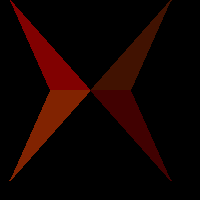
\includegraphics[width=2.2cm]{activeobjects/flipper.png} \\
        }
        &
        \makecell[l]{
          \begingroup
          \renewcommand{\arraystretch}{.8} % Default value: 1
          \begin{tabular}[t]{ll}
\tcode{Draw Routine: cdraw\_sflipper}   &    \tcode{Start address of pixel data.: 00000000}  \\
\tcode{X: -12}   &    \tcode{Colour: 00f0}  \\
\tcode{Y: -26}   &    \tcode{Scale factor: 0001}  \\
\tcode{Z: 71}   &    \tcode{0 = climb rail, 1 = cross rail, 2 = blowaway: 0000}  \\
\tcode{Position/lane on web.: 0}   &    \tcode{Size of Pixel Data: c9d20007}  \\
\tcode{Velocity: 0}   &    \tcode{Marked for deletion: 0000}  \\
\tcode{Acceleration/Flipper Mode: 00000808}   &    \tcode{Enemy or Not: enemy}  \\
\tcode{XZ Orientation  (Roll): 112}   &    \tcode{run\_vex routine: run\_flipper}  \\
\tcode{Y Rotation  (Pitch): 0}   &    \tcode{Address of Previous Object: 0000ce78}  \\
\tcode{Z Rotation  (Yaw): 0}   &    \tcode{Address of Next Object: 0000cdb8}  \\
\tcode{draw\_vex routine: draw\_vxc}   &    \tcode{Current Address: 0xce38}  \\
          \end{tabular}
          \endgroup
        }
        \\
        \toprule
        Flipper & Object Data \\
        \midrule
        \makecell[l]{
            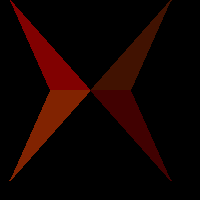
\includegraphics[width=2.2cm]{activeobjects/flipper.png} \\
        }
        &
        \makecell[l]{
          \begingroup
          \renewcommand{\arraystretch}{.8} % Default value: 1
          \begin{tabular}[t]{ll}
\tcode{Draw Routine: cdraw\_sflipper}   &    \tcode{Start address of pixel data.: 00000000}  \\
\tcode{X: -12}   &    \tcode{Colour: 00f0}  \\
\tcode{Y: -26}   &    \tcode{Scale factor: 0001}  \\
\tcode{Z: 125}   &    \tcode{0 = climb rail, 1 = cross rail, 2 = blowaway: 0000}  \\
\tcode{Position/lane on web.: 0}   &    \tcode{Size of Pixel Data: c9ce0000}  \\
\tcode{Velocity: 1}   &    \tcode{Marked for deletion: 0000}  \\
\tcode{Acceleration/Flipper Mode: 00000808}   &    \tcode{Enemy or Not: enemy}  \\
\tcode{XZ Orientation  (Roll): 112}   &    \tcode{run\_vex routine: run\_flipper}  \\
\tcode{Y Rotation  (Pitch): 0}   &    \tcode{Address of Previous Object: 0000cef8}  \\
\tcode{Z Rotation  (Yaw): 0}   &    \tcode{Address of Next Object: 0000ce38}  \\
\tcode{draw\_vex routine: draw\_vxc}   &    \tcode{Current Address: 0xce78}  \\
          \end{tabular}
          \endgroup
        }
        \\
        \bottomrule
      \end{tabular}
    \end{adjustbox}
  }
\end{figure}

\begin{figure}[H]
  {
    \setlength{\tabcolsep}{3.0pt}
    \setlength\cmidrulewidth{\heavyrulewidth} % Make cmidrule = 
    \begin{adjustbox}{center}
      \begin{tabular}[t]{ll}
        \toprule
        Spiker & Object Data \\
        \midrule
        \makecell[l]{
            
\includegraphics[width=2.2cm]{activeobjects/chevron.png} \\
        }
        &
        \makecell[l]{
          \begingroup
          \renewcommand{\arraystretch}{.8} % Default value: 1
          \begin{tabular}[t]{ll}
\tcode{Draw Routine: 0000b6c4}   &    \tcode{Start address of pixel data.: ffff000a}  \\
\tcode{X: 8}   &    \tcode{Colour: 008f}  \\
\tcode{Y: 6}   &    \tcode{Scale factor: 0001}  \\
\tcode{Z: 187}   &    \tcode{0 = climb rail, 1 = cross rail, 2 = blowaway: 0002}  \\
\tcode{Position/lane on web.: 7}   &    \tcode{Size of Pixel Data: 00070007}  \\
\tcode{Velocity: 1}   &    \tcode{Marked for deletion: 0000}  \\
\tcode{Acceleration/Flipper Mode: 0000cff8}   &    \tcode{Enemy or Not: enemy}  \\
\tcode{XZ Orientation  (Roll): 592}   &    \tcode{run\_vex routine: run\_spiker}  \\
\tcode{Y Rotation  (Pitch): 0}   &    \tcode{Address of Previous Object: 0000cff8}  \\
\tcode{Z Rotation  (Yaw): 0}   &    \tcode{Address of Next Object: 0000cfb8}  \\
\tcode{draw\_vex routine: draw}   &    \tcode{Current Address: 0xceb8}  \\
          \end{tabular}
          \endgroup
        }
        \\
        \toprule
        Fuseball & Object Data \\
        \midrule
        \makecell[l]{
            
\includegraphics[width=2.2cm]{activeobjects/fbpiece1.png} \\
            
\includegraphics[width=2.2cm]{activeobjects/fbpiece2.png} \\
        }
        &
        \makecell[l]{
          \begingroup
          \renewcommand{\arraystretch}{.8} % Default value: 1
          \begin{tabular}[t]{ll}
\tcode{Draw Routine: draw\_sfuseball}   &    \tcode{Start address of pixel data.: 00000001}  \\
\tcode{X: -16}   &    \tcode{Colour: 000f}  \\
\tcode{Y: -25}   &    \tcode{Scale factor: 0001}  \\
\tcode{Z: 163}   &    \tcode{0 = climb rail, 1 = cross rail, 2 = blowaway: 0001}  \\
\tcode{Position/lane on web.: 0}   &    \tcode{Size of Pixel Data: 30300101}  \\
\tcode{Velocity: -1}   &    \tcode{Marked for deletion: 0000}  \\
\tcode{Acceleration/Flipper Mode: 00004000}   &    \tcode{Enemy or Not: enemy}  \\
\tcode{XZ Orientation  (Roll): 526}   &    \tcode{run\_vex routine: run\_fuseball}  \\
\tcode{Y Rotation  (Pitch): 0}   &    \tcode{Address of Previous Object: 0000cf38}  \\
\tcode{Z Rotation  (Yaw): 0}   &    \tcode{Address of Next Object: 0000ce78}  \\
\tcode{draw\_vex routine: draw}   &    \tcode{Current Address: 0xcef8}  \\
          \end{tabular}
          \endgroup
        }
        \\
        \toprule
        Power-Up & Object Data \\
        \midrule
        \makecell[l]{
            
\includegraphics[width=2.2cm]{activeobjects/pwrlaser.png} \\
        }
        &
        \makecell[l]{
          \begingroup
          \renewcommand{\arraystretch}{.8} % Default value: 1
          \begin{tabular}[t]{ll}
\tcode{Draw Routine: draw\_pup1}   &    \tcode{Start address of pixel data.: fff70007}  \\
\tcode{X: 14}   &    \tcode{Colour: 0058}  \\
\tcode{Y: 0}   &    \tcode{Scale factor: 0000}  \\
\tcode{Z: 29}   &    \tcode{0 = climb rail, 1 = cross rail, 2 = blowaway: 0023}  \\
\tcode{Position/lane on web.: 8}   &    \tcode{Size of Pixel Data: 0010fffc}  \\
\tcode{Velocity: 0}   &    \tcode{Marked for deletion: 0000}  \\
\tcode{Acceleration/Flipper Mode: 00010808}   &    \tcode{Enemy or Not: not an enemy}  \\
\tcode{XZ Orientation  (Roll): -48}   &    \tcode{run\_vex routine: run\_prex}  \\
\tcode{Y Rotation  (Pitch): 0}   &    \tcode{Address of Previous Object: 0000cbb8}  \\
\tcode{Z Rotation  (Yaw): 0}   &    \tcode{Address of Next Object: 0000cef8}  \\
\tcode{draw\_vex routine: draw\_prex}   &    \tcode{Current Address: 0xcf38}  \\
          \end{tabular}
          \endgroup
        }
        \\
        \toprule
        Player Bullet & Object Data \\
        \midrule
        \makecell[l]{
            
\includegraphics[width=2.2cm]{activeobjects/bullet.png} \\
        }
        &
        \makecell[l]{
          \begingroup
          \renewcommand{\arraystretch}{.8} % Default value: 1
          \begin{tabular}[t]{ll}
\tcode{Draw Routine: draw\_pixex}   &    \tcode{Y/X in Sprite Sheet: 00b6000a}  \\
\tcode{X: 22}   &    \tcode{Colour: 0058}  \\
\tcode{Y: -16}   &    \tcode{Scale factor: 0001}  \\
\tcode{Z: 194}   &    \tcode{0 = climb rail, 1 = cross rail, 2 = blowaway: 0000}  \\
\tcode{Web Lane: 10}   &    \tcode{Width/Height in Sprite Sheet: 00070007}  \\
\tcode{Velocity: 1}   &    \tcode{Marked for deletion: ffff}  \\
\tcode{Acceleration: 0000ca72}   &    \tcode{Enemy or Not: not an enemy}  \\
\tcode{Roll: 376}   &    \tcode{run\_vex routine: player\_shot}  \\
\tcode{Pitch: 0}   &    \tcode{Address of Previous Object: ffffffff}  \\
\tcode{Yaw: 0}   &    \tcode{Address of Next Object: 0000cdf8}  \\
\tcode{draw\_vex routine: draw\_pixex}   &    \tcode{Current Address: 0xcf78}  \\
          \end{tabular}
          \endgroup
        }
        \\
        \bottomrule
      \end{tabular}
    \end{adjustbox}
  }
\end{figure}

\begin{figure}[H]
  {
    \setlength{\tabcolsep}{3.0pt}
    \setlength\cmidrulewidth{\heavyrulewidth} % Make cmidrule = 
    \begin{adjustbox}{center}
      \begin{tabular}[t]{ll}
        \toprule
        Flipper & Object Data \\
        \midrule
        \makecell[l]{
            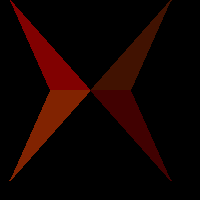
\includegraphics[width=2.2cm]{activeobjects/flipper.png} \\
        }
        &
        \makecell[l]{
          \begingroup
          \renewcommand{\arraystretch}{.8} % Default value: 1
          \begin{tabular}[t]{ll}
\tcode{Draw Routine: cdraw\_sflipper}   &    \tcode{Start address of pixel data.: 0000ffff}  \\
\tcode{X: -16}   &    \tcode{Colour: 00f0}  \\
\tcode{Y: 2}   &    \tcode{Scale factor: 0001}  \\
\tcode{Z: 55}   &    \tcode{0 = climb rail, 1 = cross rail, 2 = blowaway: 0000}  \\
\tcode{Position/lane on web.: 4}   &    \tcode{Size of Pixel Data: 00070007}  \\
\tcode{Velocity: -4}   &    \tcode{Marked for deletion: 0000}  \\
\tcode{Acceleration/Flipper Mode: 00000808}   &    \tcode{Enemy or Not: enemy}  \\
\tcode{XZ Orientation  (Roll): 16}   &    \tcode{run\_vex routine: run\_flipper}  \\
\tcode{Y Rotation  (Pitch): 0}   &    \tcode{Address of Previous Object: 0000ceb8}  \\
\tcode{Z Rotation  (Yaw): 0}   &    \tcode{Address of Next Object: 0000cbb8}  \\
\tcode{draw\_vex routine: draw\_vxc}   &    \tcode{Current Address: 0xcfb8}  \\
          \end{tabular}
          \endgroup
        }
        \\
        \toprule
        Spiker & Object Data \\
        \midrule
        \makecell[l]{
            
\includegraphics[width=2.2cm]{activeobjects/chevron.png} \\
        }
        &
        \makecell[l]{
          \begingroup
          \renewcommand{\arraystretch}{.8} % Default value: 1
          \begin{tabular}[t]{ll}
\tcode{Draw Routine: 0000b694}   &    \tcode{Start address of pixel data.: 00576000}  \\
\tcode{X: 8}   &    \tcode{Colour: 008f}  \\
\tcode{Y: 6}   &    \tcode{Scale factor: ffff}  \\
\tcode{Z: 190}   &    \tcode{0 = climb rail, 1 = cross rail, 2 = blowaway: 0000}  \\
\tcode{Position/lane on web.: 7}   &    \tcode{Size of Pixel Data: c9ca0000}  \\
\tcode{Velocity: 0}   &    \tcode{Marked for deletion: 0000}  \\
\tcode{Acceleration/Flipper Mode: 00000000}   &    \tcode{Enemy or Not: not an enemy}  \\
\tcode{XZ Orientation  (Roll): -16}   &    \tcode{run\_vex routine: run\_spike}  \\
\tcode{Y Rotation  (Pitch): 0}   &    \tcode{Address of Previous Object: 0000d038}  \\
\tcode{Z Rotation  (Yaw): 0}   &    \tcode{Address of Next Object: 0000ceb8}  \\
\tcode{draw\_vex routine: draw\_spike}   &    \tcode{Current Address: 0xcff8}  \\
          \end{tabular}
          \endgroup
        }
        \\
        \toprule
        Flipper & Object Data \\
        \midrule
        \makecell[l]{
            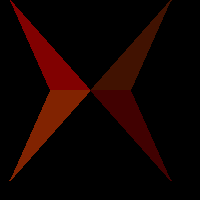
\includegraphics[width=2.2cm]{activeobjects/flipper.png} \\
        }
        &
        \makecell[l]{
          \begingroup
          \renewcommand{\arraystretch}{.8} % Default value: 1
          \begin{tabular}[t]{ll}
\tcode{Draw Routine: cdraw\_sflipper}   &    \tcode{Start address of pixel data.: 00000000}  \\
\tcode{X: 0}   &    \tcode{Colour: 00f0}  \\
\tcode{Y: 8}   &    \tcode{Scale factor: 0001}  \\
\tcode{Z: 330}   &    \tcode{0 = climb rail, 1 = cross rail, 2 = blowaway: 0000}  \\
\tcode{Position/lane on web.: 6}   &    \tcode{Size of Pixel Data: 00100000}  \\
\tcode{Velocity: 0}   &    \tcode{Marked for deletion: 0000}  \\
\tcode{Acceleration/Flipper Mode: 00000808}   &    \tcode{Enemy or Not: enemy}  \\
\tcode{XZ Orientation  (Roll): 0}   &    \tcode{run\_vex routine: run\_flipper}  \\
\tcode{Y Rotation  (Pitch): 0}   &    \tcode{Address of Previous Object: 0000cbf8}  \\
\tcode{Z Rotation  (Yaw): 0}   &    \tcode{Address of Next Object: 0000cff8}  \\
\tcode{draw\_vex routine: fffd}   &    \tcode{Current Address: 0xd038}  \\
          \end{tabular}
          \endgroup
        }
        \\
        \toprule
        Player Bullet & Object Data \\
        \midrule
        \makecell[l]{
            
\includegraphics[width=2.2cm]{activeobjects/bullet.png} \\
        }
        &
        \makecell[l]{
          \begingroup
          \renewcommand{\arraystretch}{.8} % Default value: 1
          \begin{tabular}[t]{ll}
\tcode{Draw Routine: draw\_pixex}   &    \tcode{Y/X in Sprite Sheet: 00b6000a}  \\
\tcode{X: 26}   &    \tcode{Colour: 0028}  \\
\tcode{Y: -24}   &    \tcode{Scale factor: 0001}  \\
\tcode{Z: 191}   &    \tcode{0 = climb rail, 1 = cross rail, 2 = blowaway: 0000}  \\
\tcode{Web Lane: 11}   &    \tcode{Width/Height in Sprite Sheet: 00070007}  \\
\tcode{Velocity: 1}   &    \tcode{Marked for deletion: ffff}  \\
\tcode{Acceleration: 0000ca86}   &    \tcode{Enemy or Not: not an enemy}  \\
\tcode{Roll: 368}   &    \tcode{run\_vex routine: player\_shot}  \\
\tcode{Pitch: 0}   &    \tcode{Address of Previous Object: 0000cb78}  \\
\tcode{Yaw: 0}   &    \tcode{Address of Next Object: 0000ccb8}  \\
\tcode{draw\_vex routine: draw\_pixex}   &    \tcode{Current Address: 0xd078}  \\
          \end{tabular}
          \endgroup
        }
        \\
        \bottomrule
      \end{tabular}
    \end{adjustbox}
  }
\end{figure}
